%
% This is an example LaTeX file which uses the SANDreport class file.
% It shows how a SAND report should be formatted, what sections and
% elements it should contain, and how to use the SANDreport class.
% It uses the LaTeX article class, but not the strict option.
% ItINLreport uses .eps logos and files to show how pdflatex can be used
%
% Get the latest version of the class file and more at
%    http://www.cs.sandia.gov/~rolf/SANDreport
%
% This file and the SANDreport.cls file are based on information
% contained in "Guide to Preparing {SAND} Reports", Sand98-0730, edited
% by Tamara K. Locke, and the newer "Guide to Preparing SAND Reports and
% Other Communication Products", SAND2002-2068P.
% Please send corrections and suggestions for improvements to
% Rolf Riesen, Org. 9223, MS 1110, rolf@cs.sandia.gov
%

\documentclass[pdf,12pt]{INLreport}
% pslatex is really old (1994).  It attempts to merge the times and mathptm packages.
% My opinion is that it produces a really bad looking math font.  So why are we using it?
% If you just want to change the text font, you should just \usepackage{times}.
% \usepackage{pslatex}
\usepackage{times}
\usepackage[FIGBOTCAP,normal,bf,tight]{subfigure}
\usepackage{amsmath}
\usepackage{amssymb}
\usepackage{soul}
\usepackage{pifont}
\usepackage{enumerate}
\usepackage{listings}
\usepackage{fullpage}
\usepackage{xcolor}          % Using xcolor for more robust color specification
\usepackage{ifthen}          % For simple checking in newcommand blocks
\usepackage{textcomp}
\usepackage{mathtools}
\usepackage{relsize}
\usepackage{lscape}
\usepackage[toc,page]{appendix}

\graphicspath{{./figures/}}

\newtheorem{mydef}{Definition}
\newcommand{\norm}[1]{\lVert#1\rVert}
%\usepackage[table,xcdraw]{xcolor}
%\usepackage{authblk}         % For making the author list look prettier
%\renewcommand\Authsep{,~\,}

% Custom colors
\definecolor{deepblue}{rgb}{0,0,0.5}
\definecolor{deepred}{rgb}{0.6,0,0}
\definecolor{deepgreen}{rgb}{0,0.5,0}
\definecolor{forestgreen}{RGB}{34,139,34}
\definecolor{orangered}{RGB}{239,134,64}
\definecolor{darkblue}{rgb}{0.0,0.0,0.6}
\definecolor{gray}{rgb}{0.4,0.4,0.4}

\lstset {
  basicstyle=\ttfamily,
  frame=single
}


\setcounter{secnumdepth}{5}
\lstdefinestyle{XML} {
    language=XML,
    extendedchars=true,
    breaklines=true,
    breakatwhitespace=true,
%    emph={name,dim,interactive,overwrite},
    emphstyle=\color{red},
    basicstyle=\ttfamily,
%    columns=fullflexible,
    commentstyle=\color{gray}\upshape,
    morestring=[b]",
    morecomment=[s]{<?}{?>},
    morecomment=[s][\color{forestgreen}]{<!--}{-->},
    keywordstyle=\color{cyan},
    stringstyle=\ttfamily\color{black},
    tagstyle=\color{darkblue}\bf\ttfamily,
    morekeywords={name,type},
%    morekeywords={name,attribute,source,variables,version,type,release,x,z,y,xlabel,ylabel,how,text,param1,param2,color,label},
}
\lstset{language=python,upquote=true}

\usepackage{titlesec}
\newcommand{\sectionbreak}{\clearpage}
\setcounter{secnumdepth}{4}

%\titleformat{\paragraph}
%{\normalfont\normalsize\bfseries}{\theparagraph}{1em}{}
%\titlespacing*{\paragraph}
%{0pt}{3.25ex plus 1ex minus .2ex}{1.5ex plus .2ex}

%%%%%%%% Begin comands definition to input python code into document
\usepackage[utf8]{inputenc}

% Default fixed font does not support bold face
\DeclareFixedFont{\ttb}{T1}{txtt}{bx}{n}{9} % for bold
\DeclareFixedFont{\ttm}{T1}{txtt}{m}{n}{9}  % for normal

\usepackage{listings}

% Python style for highlighting
\newcommand\pythonstyle{\lstset{
language=Python,
basicstyle=\ttm,
otherkeywords={self, none, return},             % Add keywords here
keywordstyle=\ttb\color{deepblue},
emph={MyClass,__init__},          % Custom highlighting
emphstyle=\ttb\color{deepred},    % Custom highlighting style
stringstyle=\color{deepgreen},
frame=tb,                         % Any extra options here
showstringspaces=false            %
}}


% Python environment
\lstnewenvironment{python}[1][]
{
\pythonstyle
\lstset{#1}
}
{}

% Python for external files
\newcommand\pythonexternal[2][]{{
\pythonstyle
\lstinputlisting[#1]{#2}}}

\lstnewenvironment{xml}
{}
{}

% Python for inline
\newcommand\pythoninline[1]{{\pythonstyle\lstinline!#1!}}


\def\DRAFT{} % Uncomment this if you want to see the notes people have been adding
% Comment command for developers (Should only be used under active development)
\ifdefined\DRAFT
  \newcommand{\nameLabeler}[3]{\textcolor{#2}{[[#1: #3]]}}
\else
  \newcommand{\nameLabeler}[3]{}
\fi
% Commands for making the LaTeX a bit more uniform and cleaner
\newcommand{\TODO}[1]    {\textcolor{red}{\textit{(#1)}}}
\newcommand{\xmlAttrRequired}[1] {\textcolor{red}{\textbf{\texttt{#1}}}}
\newcommand{\xmlAttr}[1] {\textcolor{cyan}{\textbf{\texttt{#1}}}}
\newcommand{\xmlNodeRequired}[1] {\textcolor{deepblue}{\textbf{\texttt{<#1>}}}}
\newcommand{\xmlNode}[1] {\textcolor{darkblue}{\textbf{\texttt{<#1>}}}}
\newcommand{\xmlString}[1] {\textcolor{black}{\textbf{\texttt{'#1'}}}}
\newcommand{\xmlDesc}[1] {\textbf{\textit{#1}}} % Maybe a misnomer, but I am
                                                % using this to detail the data
                                                % type and necessity of an XML
                                                % node or attribute,
                                                % xmlDesc = XML description
\newcommand{\default}[1]{~\\*\textit{Default: #1}}
\newcommand{\nb} {\textcolor{deepgreen}{\textbf{~Note:}}~}
\newcommand{\ppType}[2]
{
  In order to use the \textit{#1} PP, the user needs to set the
  \xmlAttr{subType} of a \xmlNode{PostProcessor} node:

  \xmlNode{PostProcessor \xmlAttr{name}=\xmlString{ppName} \xmlAttr{subType}=\xmlString{SR2ML.#2}/}.

   Several sub-nodes are available:
}

%%%%%%%% End comands definition to input python code into document

%\usepackage[dvips,light,first,bottomafter]{draftcopy}
%\draftcopyName{Sample, contains no OUO}{70}
%\draftcopyName{Draft}{300}

% The bm package provides \bm for bold math fonts.  Apparently
% \boldsymbol, which I used to always use, is now considered
% obsolete.  Also, \boldsymbol doesn't even seem to work with
% the fonts used in this particular document...
\usepackage{bm}


% Define tensors to be in bold math font.
\newcommand{\tensor}[1]{{\bm{#1}}}

% Override the formatting used by \vec.  Instead of a little arrow
% over the letter, this creates a bold character.
\renewcommand{\vec}{\bm}

% Define unit vector notation.  If you don't override the
% behavior of \vec, you probably want to use the second one.
\newcommand{\unit}[1]{\hat{\bm{#1}}}
% \newcommand{\unit}[1]{\hat{#1}}

% Use this to refer to a single component of a unit vector.
\newcommand{\scalarunit}[1]{\hat{#1}}

% \toprule, \midrule, \bottomrule for tables
\usepackage{booktabs}

% \llbracket, \rrbracket
\usepackage{stmaryrd}

\usepackage{hyperref}
\hypersetup{
    colorlinks,
    citecolor=black,
    filecolor=black,
    linkcolor=black,
    urlcolor=black
}

% Compress lists of citations like [33,34,35,36,37] to [33-37]
\usepackage{cite}

% If you want to relax some of the SAND98-0730 requirements, use the "relax"
% option. It adds spaces and boldface in the table of contents, and does not
% force the page layout sizes.
% e.g. \documentclass[relax,12pt]{SANDreport}
%
% You can also use the "strict" option, which applies even more of the
% SAND98-0730 guidelines. It gets rid of section numbers which are often
% useful; e.g. \documentclass[strict]{SANDreport}

% The INLreport class uses \flushbottom formatting by default (since
% it's intended to be two-sided document).  \flushbottom causes
% additional space to be inserted both before and after paragraphs so
% that no matter how much text is actually available, it fills up the
% page from top to bottom.  My feeling is that \raggedbottom looks much
% better, primarily because most people will view the report
% electronically and not in a two-sided printed format where some argue
% \raggedbottom looks worse.  If we really want to have the original
% behavior, we can comment out this line...
\raggedbottom
\setcounter{secnumdepth}{5} % show 5 levels of subsection
\setcounter{tocdepth}{5} % include 5 levels of subsection in table of contents

% ---------------------------------------------------------------------------- %
%
% Set the title, author, and date
%
\title{SR2ML User Manual}
%\author{%
%\begin{tabular}{c} Author 1 \\ University1 \\ Mail1 \\ \\
%Author 3 \\ University3 \\ Mail3 \end{tabular} \and
%\begin{tabular}{c} Author 2 \\ University2 \\ Mail2 \\ \\
%Author 4 \\ University4 \\ Mail4\\
%\end{tabular} }


\author{
\\Diego Mandelli
\\Congjian Wang
}

% There is a "Printed" date on the title page of a SAND report, so
% the generic \date should [WorkingDir:]generally be empty.
\date{}


% ---------------------------------------------------------------------------- %
% Set some things we need for SAND reports. These are mandatory
%
\SANDnum{INL/EXT-20-57857}
\SANDprintDate{\today}
\SANDauthor{Congjian Wang and Diego Mandelli}
\SANDreleaseType{Revision 1}
\def\component#1{\texttt{#1}}

% ---------------------------------------------------------------------------- %
\newcommand{\systemtau}{\tensor{\tau}_{\!\text{SUPG}}}

\usepackage{placeins}
\usepackage{array}

\newcolumntype{L}[1]{>{\raggedright\let\newline\\\arraybackslash\hspace{0pt}}m{#1}}
\newcolumntype{C}[1]{>{\centering\let\newline\\\arraybackslash\hspace{0pt}}m{#1}}
\newcolumntype{R}[1]{>{\raggedleft\let\newline\\\arraybackslash\hspace{0pt}}m{#1}}

% ---------------------------------------------------------------------------- %
%
% Start the document
%
\begin{document}
    \maketitle

    % ------------------------------------------------------------------------ %
    % The table of contents and list of figures and tables
    % Comment out \listoffigures and \listoftables if there are no
    % figures or tables. Make sure this starts on an odd numbered page
    %
    \cleardoublepage		% TOC needs to start on an odd page
    \tableofcontents
    %\listoffigures
    %\listoftables
    % ---------------------------------------------------------------------- %
    \SANDmain

    % ---------------------------------------------------------------------- %
    % This is where the body of the report begins; usually with an Introduction
    %
    section{Introduction}
\label{sec:Introduction}

SR2ML is a software package which contains a set of safety and reliability models
designed to be interfaced with the INL developed RAVEN code. These models can be
employed to perform both static and dynamic system risk analysis and determine
risk importance of specific elements of the considered system.

Two classes of reliability models have been developed; the first class includes
all classical reliability models (Fault-Trees, Event-Trees, Markov models and
Reliability Block Diagrams) which have been extended to deal not only with
Boolean logic values but also time dependent values. The second class includes
several components aging and maintenance models. Models of these two classes are designed to
be included in a RAVEN ensemble model to perform time dependent system reliability
analysis (dynamic analysis). Similarly, these models can be interfaced with system
analysis codes  to determine failure time of systems and evaluate accident progression
(static analysis).

\subsection{Acquiring and Installing SR2ML}
SR2ML is supported on three separate computing platforms: Linux, OSX (Apple Macintosh), and Microsoft
Windows. Currently, SR2ML is downloadable from the SR2ML GitLab repository:
\url{https://hpcgitlab.hpc.inl.gov/RAVEN_PLUGINS/SR2ML.git}. New users should contact SR2ML developers to
get started with SR2ML. This typically involves the following steps:

\begin{itemize}
  \item \textit{Download SR2ML}
    \\ You can download the source code for SR2ML from \url{https://hpcgitlab.hpc.inl.gov/RAVEN_PLUGINS/SR2ML.git}.
	\item \textit{Use as a RAVEN Plugin}, RAVEN must first be downloaded from
  \url{https://github.com/idaholab/raven.git}.
		\\ Detailed instructions are available from \url{https://github.com/idaholab/raven/wiki}.
    To register a plugin with RAVEN and make its components accessible, run the script:
    \begin{lstlisting}[language=bash]
  	raven/scripts/install_plugins.py -s /abs/path/to/SR2ML
  	\end{lstlisting}
    After the plugin registration, then following the installation instruction at
    \url{https://github.com/idaholab/raven/wiki/installationMain} to install the
    required dependencies.
\end{itemize}

\subsection{User Manual Formats}
In this manual, we employ the following formats to highlight certain parts with
particular meanings (i.e. input structure, examples, and terminal commands):

\begin{itemize}
\item \textbf{\textit{Python Coding:}}
\begin{lstlisting}[language=python]
class AClass():
  def aMethodImplementation(self):
    pass
\end{lstlisting}
\item \textbf{\textit{SR2ML XML input example:}}
\begin{lstlisting}[style=XML,morekeywords={anAttribute}]
<MainXMLBlock>
  ...
  <aXMLnode anAttribute='aValue'>
     <aSubNode>body</aSubNode>
  </aXMLnode>
  <!-- This is  commented block -->
  ...
</MainXMLBlock>
\end{lstlisting}
\item \textbf{\textit{Bash Commands:}}
\begin{lstlisting}[language=bash]
cd path/to/SR2ML/
cd ../../
\end{lstlisting}
\end{itemize}

\subsection{Capabilities of SR2ML}
This document provides a detailed description of the SR2ML plugin for the RAVEN~\cite{RAVEN,RAVENtheoryMan} code.
The features included in this plugin are:
\begin{itemize}
	\item Event Tree (ET) Model (see Section~\ref{sec:ETModel})
	\item Fault Tree (FT) Model (see Section~\ref{sec:FTModel})
	\item Markov Model (see Section~\ref{sec:MarkovModel})
	\item Reliability Block Diagram (RBD) Model (see Section~\ref{sec:RBDmodel})
	\item Data Classifier (see Section~\ref{sec:dataClassifier})
	\item ET Data Importer (see Section~\ref{sec:ETdataImporter})
	\item FT Data Importer (see Section~\ref{sec:FTdataImporter})
	\item Reliability Models (see Section~\ref{sec:ReliabilityModels})
  \item Maintenance Models (see Section~\ref{sec:MaintenanceModels})
\end{itemize}

    %%%%%%%%%%%%% External Models %%%%%%%%%%%%%%
    \section{ET Model}
\label{sec:ETModel}

This model is designed to read from file the structure of the ET and to import such Boolean logic structure as a RAVEN model.
The ET must be specified in a specific format: the OpenPSA format (\href{<url>}{https://github.com/open-psa}).
As an example, the ET of Fig.~\ref{fig:ET} is translated in the OpenPSA format as shown below:

\begin{lstlisting}[style=XML,morekeywords={anAttribute},caption=ET of Fig.~\ref{fig:ET} in OpenPSA format., label=lst:ETModel]
<define-event-tree name="eventTree">
    <define-functional-event name="ACC"/>
    <define-functional-event name="LPI"/>
    <define-functional-event name="LPR"/>
    <define-sequence name="1"/>
    <define-sequence name="2"/>
    <define-sequence name="3"/>
    <define-sequence name="4"/>
    <initial-state>
        <fork functional-event="ACC">
            <path state="0">
                <fork functional-event="LPI">
                    <path state="0">
                        <fork functional-event="LPR">
                            <path state="0">
                                <sequence name="1"/>
                            </path>
                            <path state="+1">
                                <sequence name="2"/>
                            </path>
                        </fork>
                    </path>
                    <path state="+1">
                        <sequence name="3"/>
                    </path>
                </fork>
            </path>
            <path state="+1">
                <sequence name="4"/>
            </path>
        </fork>
    </initial-state>
</define-event-tree>
\end{lstlisting}

\begin{figure}
    \centering
    \centerline{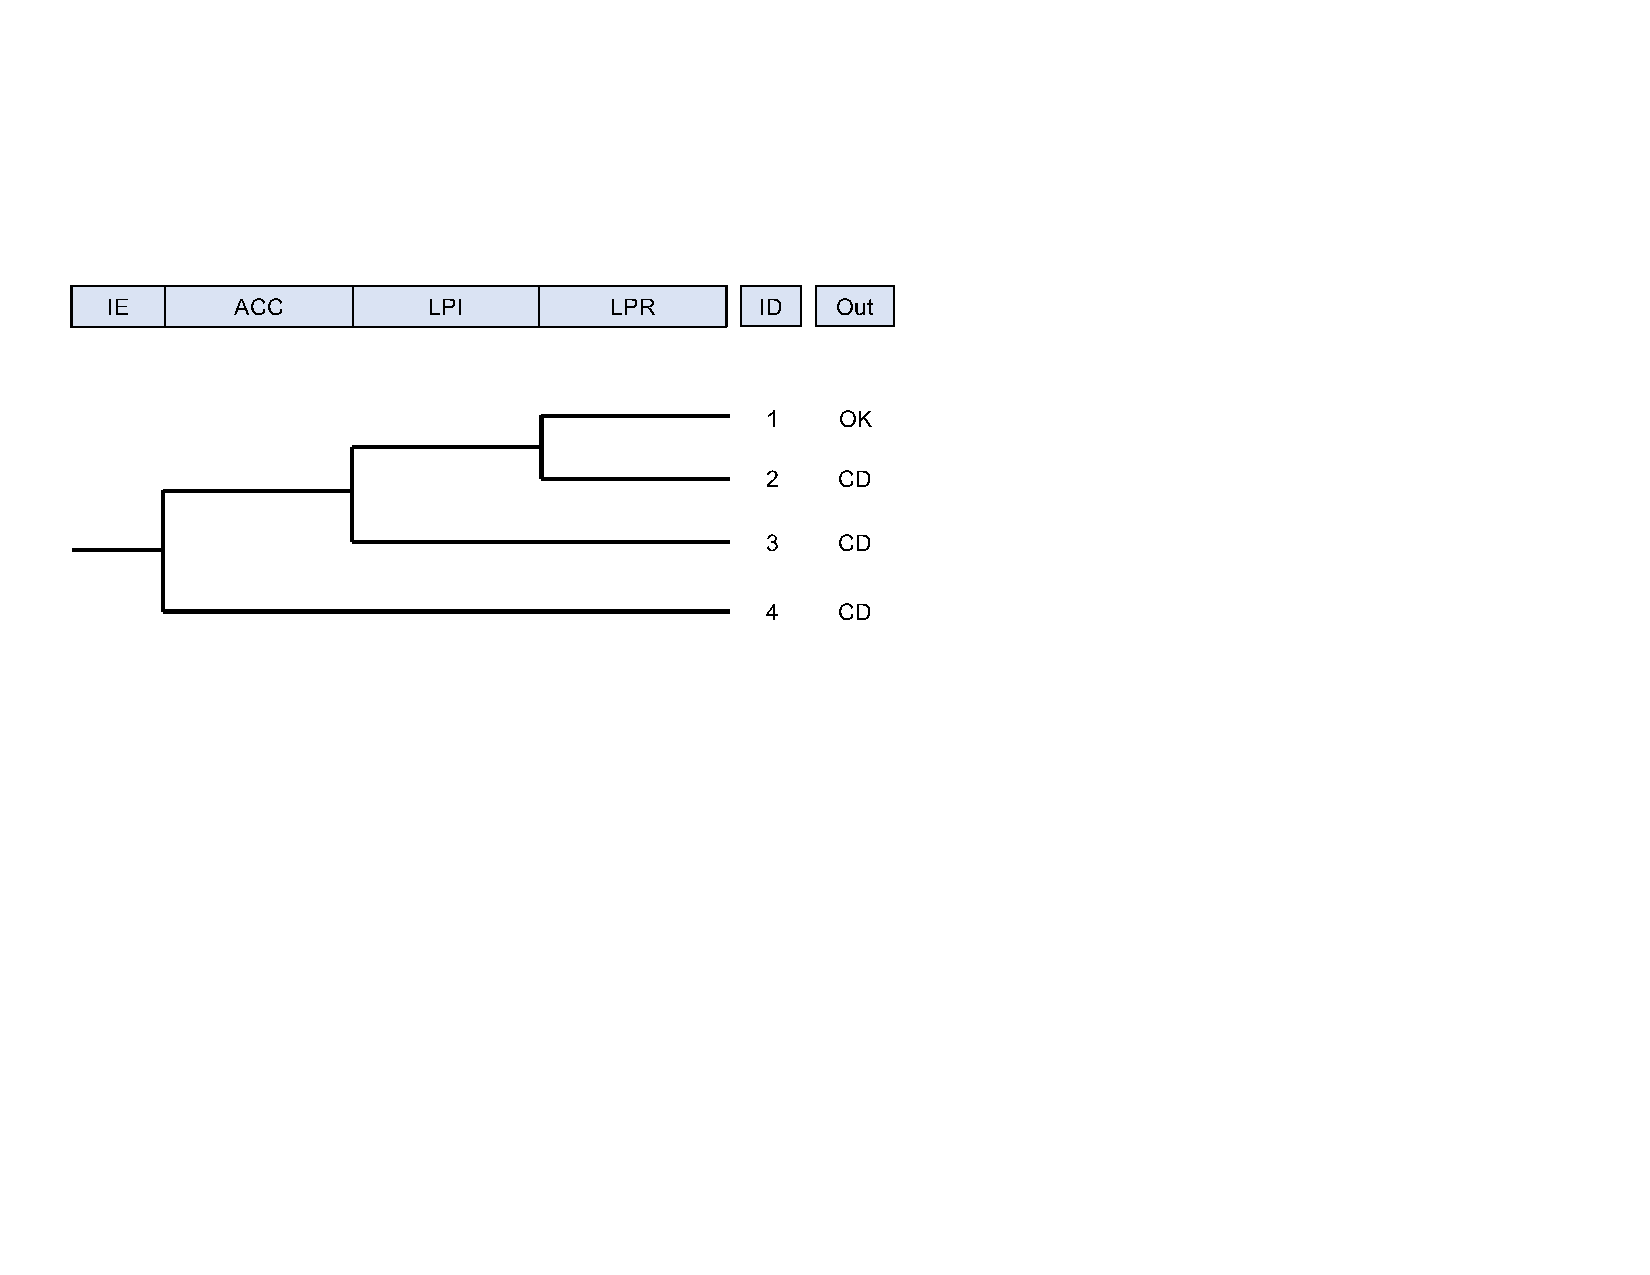
\includegraphics[scale=0.5]{ET.pdf}}
    \caption{Example of ET.}
    \label{fig:ET}
\end{figure}

The ET of Fig.~\ref{fig:ET} and defined in Listing~\ref{lst:ETModel} can be defined in the RAVEN input file as follows:
\begin{lstlisting}[style=XML,morekeywords={anAttribute},caption=ET model input example., label=lst:ET_InputExample]
  <Models>
    ...
    <ExternalModel name="ET" subType="ETModel">
      <variables>
        statusACC,statusLPI,statusLPR,sequence
      </variables>
      <map var="statusACC">ACC</map>
      <map var="statusLPI">LPI</map>
      <map var="statusLPR">LPR</map>
      <sequenceID>sequence</sequenceID>
    </ExternalModel>
    ...
  </Models>
\end{lstlisting}

All the specifications of the ET model are given in the
\xmlNode{ExternalModel} block.
Inside the \xmlNode{ExternalModel} block, the XML
nodes that belong to this models are:
\begin{itemize}
  \item  \xmlNode{variables}, \xmlDesc{string, required parameter}, a list containing the names of both the input and output variables of the model
  \item  \xmlNode{sequenceID},\xmlDesc{string, required parameter}, the name of the alias variable that indicate the branch ID
  \item  \xmlNode{map},\xmlDesc{string, required parameter}, the name ID of the ET branching variable
	  \begin{itemize}
	    \item \xmlAttr{var}, \xmlDesc{required string attribute}, the ALIAS name ID of the ET branching variable
	  \end{itemize}
\end{itemize}

Provided this definition and the ET model of Fig.~\ref{fig:ET} and described in Listing~\ref{lst:ETModel},
the resulting model in RAVEN is characterized by these variables:
\begin{itemize}
	\item Input variables: statusACC, statusLPI, statusLPR
	\item Output variable: sequence
\end{itemize}

\subsection{ET model reference tests}
\begin{itemize}
	\item SR2ML/tests/test\_ETmodel.xml
	\item SR2ML/tests/test\_ETmodel\_TD.xml
\end{itemize}

    \section{FT Model}
\label{sec:FTModel}

This model is designed to read from file the structure of the fault tree (FT) and to import such Boolean logic structure as a RAVEN model.
The FT must be specified in: the OpenPSA format (\href{<url>}{https://github.com/open-psa}).
As an example, the FT of Fig.~\ref{fig:FT} is translated in the OpenPSA as shown below:

\begin{lstlisting}[style=XML,morekeywords={anAttribute},caption=FT in OpenPSA format., label=lst:FTModel]
<opsa-mef>
    <define-fault-tree name="FT">
        <define-gate name="TOP">
            <or>
                <gate name="G1"/>
                <gate name="G2"/>
                <gate name="G3"/>
            </or>
        </define-gate>
        <define-component name="A">
            <define-gate name="G1">
                <and>
                    <basic-event name="BE1"/>
                    <basic-event name="BE2"/>
                </and>
            </define-gate>
            <define-gate name="G2">
                <and>
                    <basic-event name="BE1"/>
                    <basic-event name="BE3"/>
                </and>
            </define-gate>
            <define-basic-event name="BE1">
                <float value="1.2e-3"/>
            </define-basic-event>
            <define-component name="B">
                <define-basic-event name="BE2">
                    <float value="2.4e-3"/>
                </define-basic-event>
                <define-basic-event name="BE3">
                    <float value="5.2e-3"/>
                </define-basic-event>
            </define-component>
        </define-component>
        <define-component name="C">
            <define-gate name="G3">
                <and>
                    <basic-event name="BE1"/>
                    <basic-event name="BE4"/>
                </and>
            </define-gate>
            <define-basic-event name="BE4">
                <float value="1.6e-3"/>
            </define-basic-event>
        </define-component>
    </define-fault-tree>
</opsa-mef>
\end{lstlisting}

\begin{figure}
    \centering
    \centerline{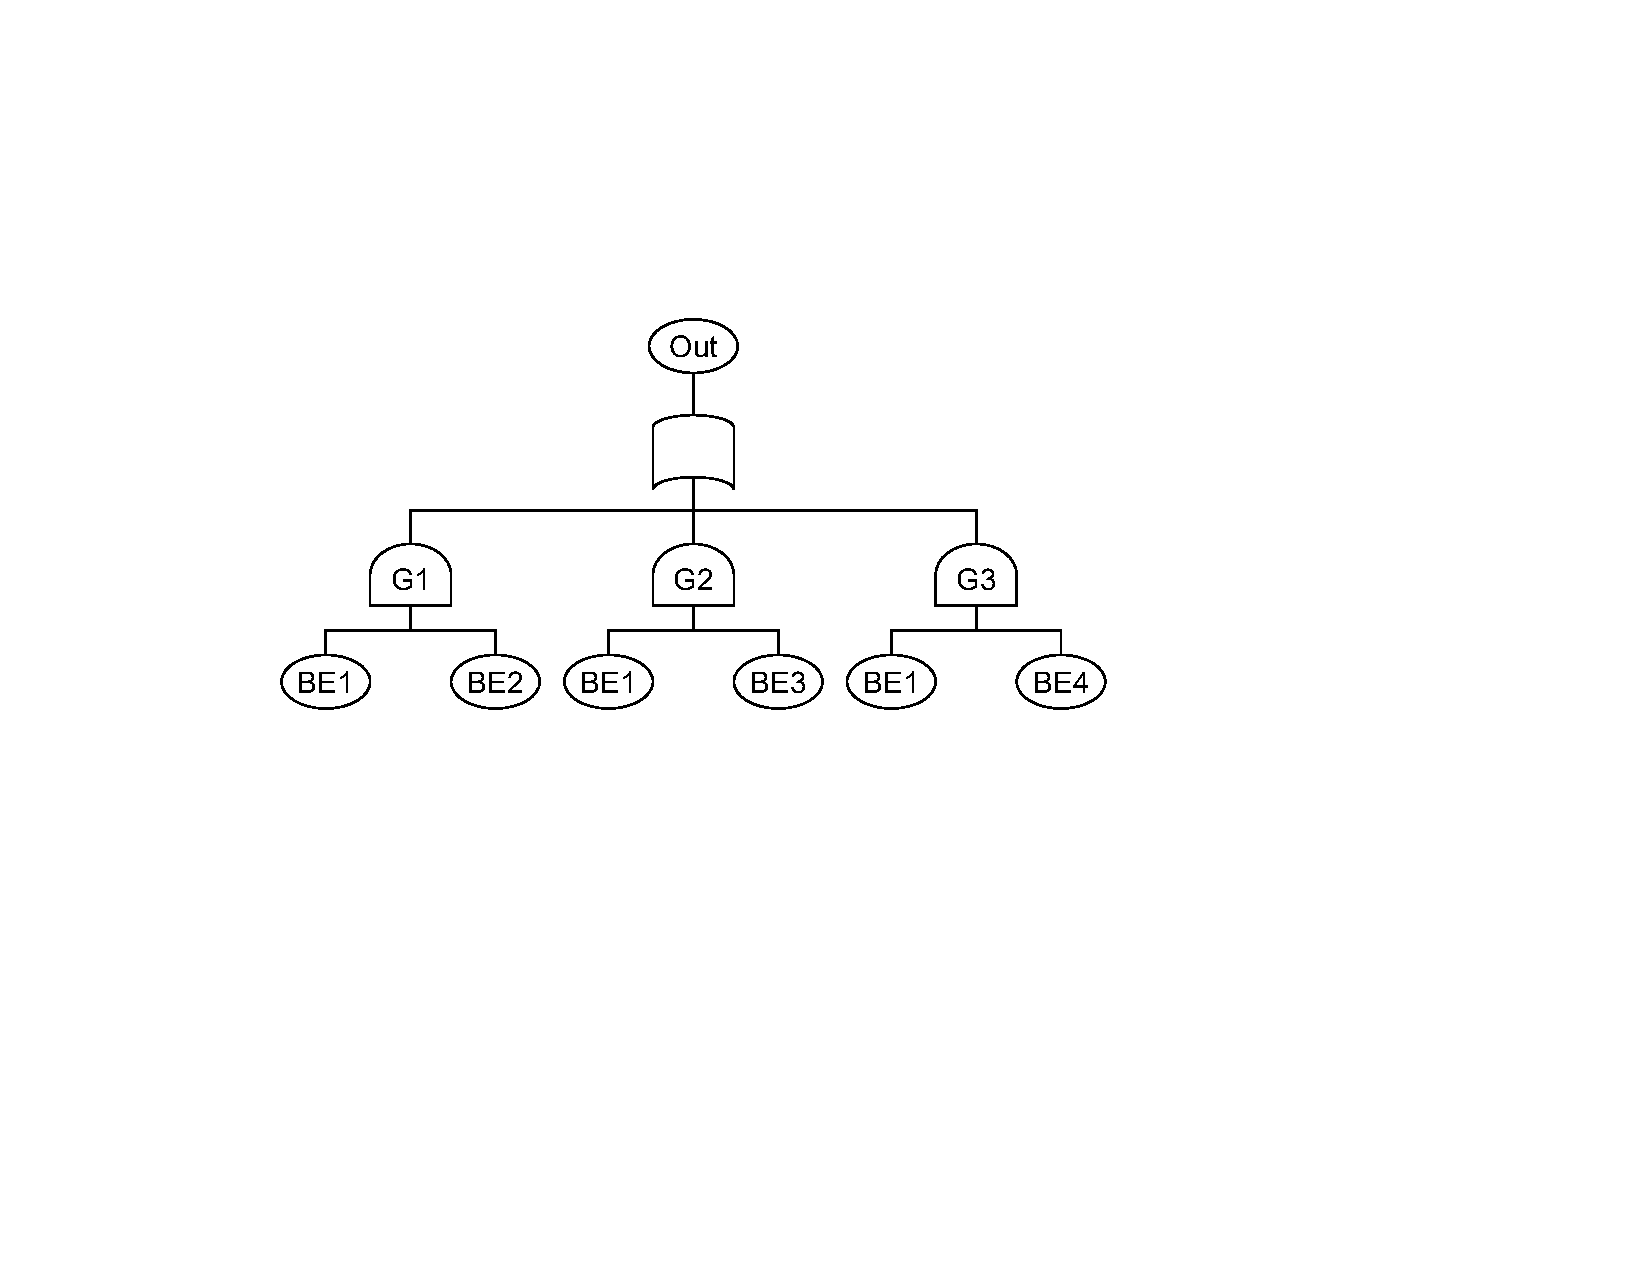
\includegraphics[scale=0.5]{FT.pdf}}
    \caption{Example of FT.}
    \label{fig:FT}
\end{figure}

The FT of Fig.~\ref{fig:FT} and defined in Listing~\ref{lst:FTModel} can be defined in the RAVEN input file as follows:

\begin{lstlisting}[style=XML,morekeywords={anAttribute},caption=FT model input example., label=lst:FT_InputExample]
  <Models>
    ...
    <ExternalModel name="FT" subType="FTModel">
      <variables>
        statusBE1,statusBE2,statusBE3,statusBE4,TOP
      </variables>
      <topEvents>TOP</topEvents>
      <map var="statusBE1">BE1</map>
      <map var="statusBE2">BE2</map>
      <map var="statusBE3">BE3</map>
      <map var="statusBE4">BE4</map>
    </ExternalModel>
    ...
  </Models>
\end{lstlisting}

All the specifications of the FT model are given in the
\xmlNode{ExternalModel} block.
Inside the \xmlNode{ExternalModel} block, the XML
nodes that belong to this models are:
\begin{itemize}
  \item  \xmlNode{variables}, \xmlDesc{string, required parameter}, a list containing the names of both the input and output variables of the model
  \item  \xmlNode{topEvents}, \xmlDesc{string, required parameter}, the name of the alias Top Event
  \item  \xmlNode{map}, \xmlDesc{string, required parameter}, the name ID of the FT basic events
	  \begin{itemize}
	    \item \xmlAttr{var}, \xmlDesc{required string attribute}, the ALIAS name ID of the FT basic events
	  \end{itemize}
\end{itemize}

Provided this definition, the FT model of Fig.~\ref{fig:FT} and described in Listing~\ref{lst:FTmodel},
the resulting model in RAVEN is characterized by these variables:
\begin{itemize}
	\item Input variables: statusBE1, statusBE2, statusBE3, statusBE4
	\item Output variable: TOP
\end{itemize}

\subsection{FT model reference tests}
\begin{itemize}
	\item SR2ML/tests/test\_FTmodel.xml
	\item SR2ML/tests/test\_FTmodel\_TD.xml
\end{itemize}

    \section{Markov Model}
\label{sec:MarkovModel}

This model is designed to import a generic Markov chain as a RAVEN model.
As an example, the Markov chain of Fig.~\ref{fig:markov} is translated in the OpenPSA as shown below:

\begin{figure}
    \centering
    \centerline{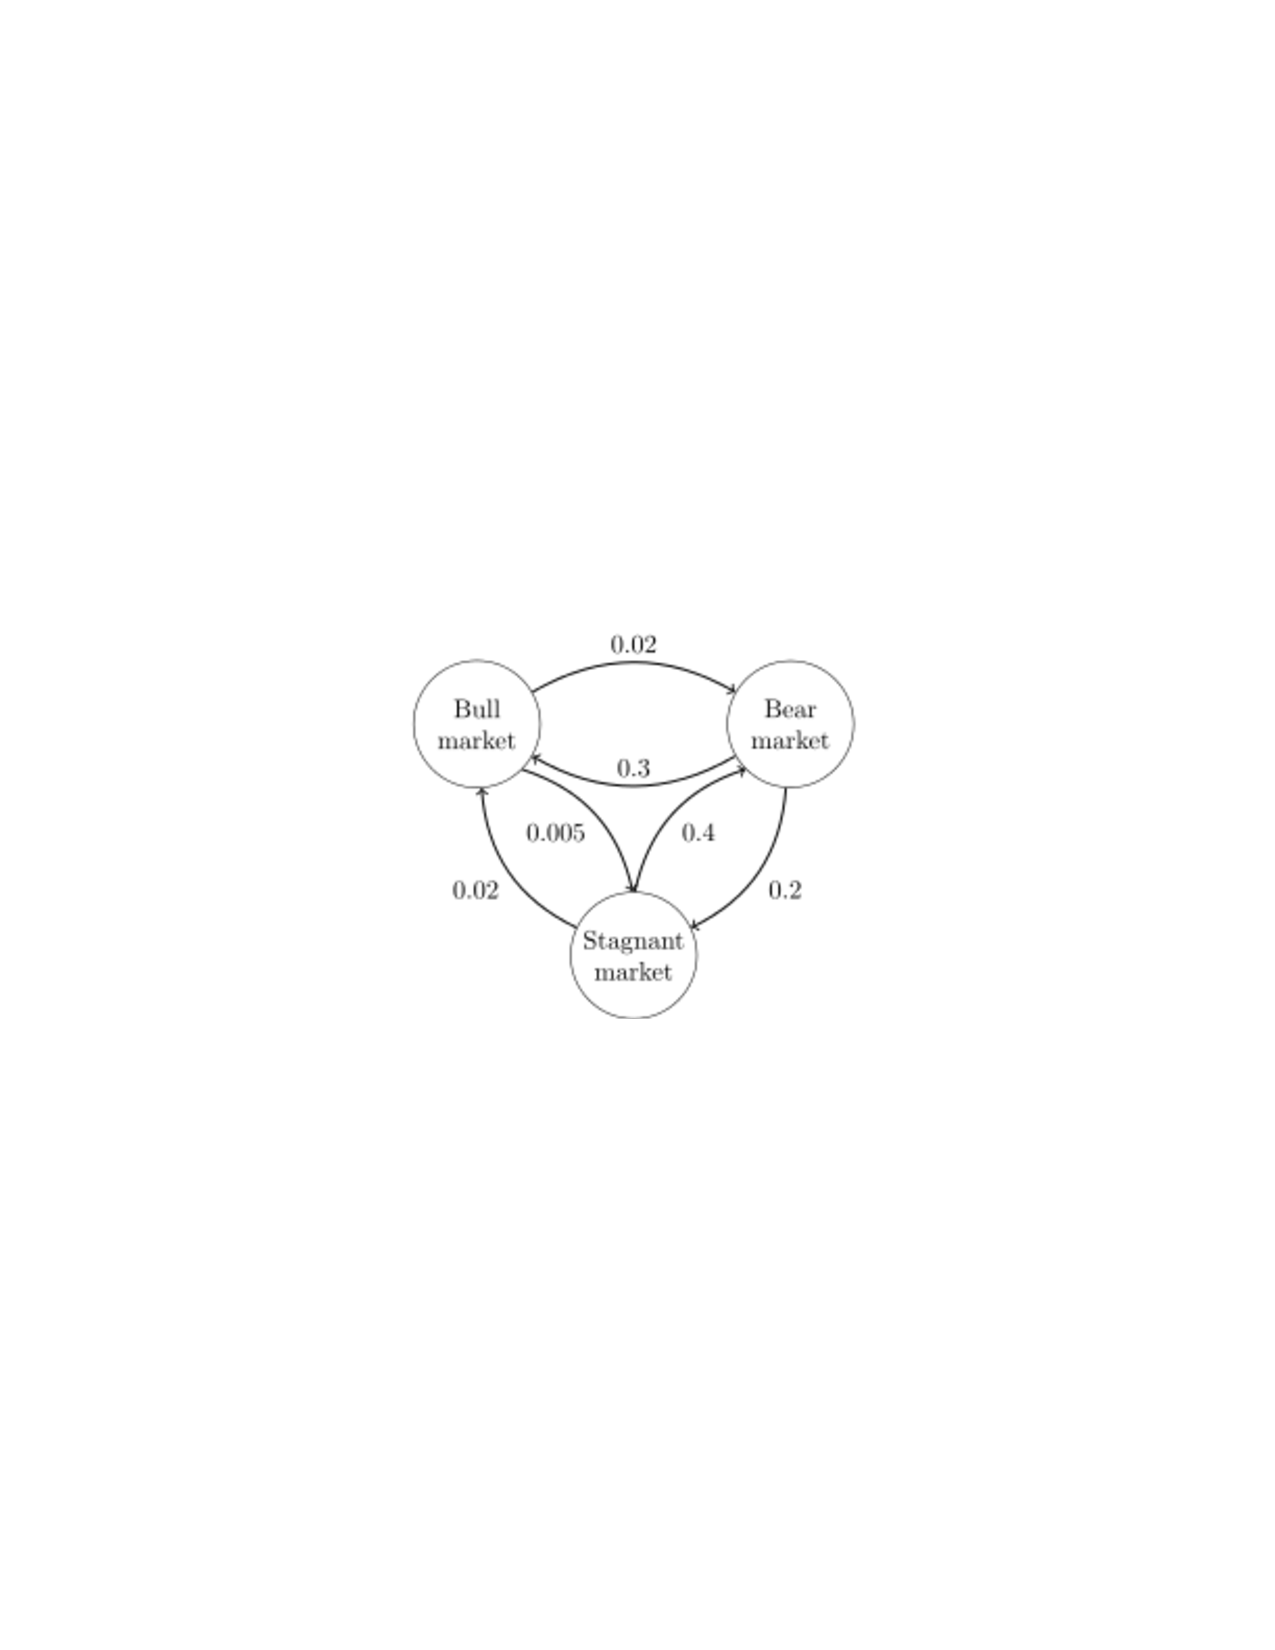
\includegraphics[scale=0.5]{markov.pdf}}
    \caption{Example of continuous time Markov chain (source Wikipedia: https://en.wikipedia.org/wiki/Markov\_chain).}
    \label{fig:markov}
\end{figure}

\begin{lstlisting}[style=XML,morekeywords={anAttribute},caption=Markov model input example., label=lst:Markov_InputExample]
  <Models>
    <ExternalModel name="markov" subType="MarkovModel">
      <variables>initialState,finalState</variables>
      <initState>initialState</initState>
      <finState>finalState</finState>
      <endTime>1000</endTime>
      <state name="1"> <!-- Bull market -->
        <transition type="lambda" value="0.02" >2</transition>
        <transition type="lambda" value="0.005">3</transition>
      </state>
      <state name="2"> <!-- Bear market -->
        <transition type="lambda" value="0.3">1</transition>
        <transition type="lambda" value="0.2">3</transition>
      </state>
      <state name="3"> <!-- Stagnant market -->
        <transition type="lambda" value="0.02">1</transition>
        <transition type="lambda" value="0.4" >2</transition>
      </state>
    </ExternalModel>
  </Models>
\end{lstlisting}

All the specifications of the Markov model are given in the \xmlNode{ExternalModel} block.
Inside the \xmlNode{ExternalModel} block, the XML nodes that belong to this model are:
\begin{itemize}
  \item  \xmlNode{variables}, \xmlDesc{string, required parameter}, a list containing the names of both the input and output variables of the model
  \item  \xmlNode{initState}, \xmlDesc{string, required parameter}, variable ID corresponding to initial state
  \item  \xmlNode{finState}, \xmlDesc{string, required parameter}, variable ID corresponding to final state
  \item  \xmlNode{endTime}, \xmlDesc{float, required parameter}, time horizon to evaluate Markov chain transition history
  \item  \xmlNode{state}, specifies a single node; inside a \xmlNode{state} all possible transitions OUT of this state must be specified in the \xmlNode{transition} xml sub-nodes:
	  \begin{itemize}
	  	\item \xmlAttr{transition}, \xmlDesc{required string attribute}, arrival state
	    \item \xmlAttr{type}, \xmlDesc{required string attribute}, type of transition. Allowed transition types are:
      lambda, tau, instant and unif (see below)
	    \item \xmlAttr{value}, \xmlDesc{required string attribute}, value associated to the particular transition.
	  \end{itemize}
\end{itemize}

The following transition types are available:
\begin{itemize}
  \item \textbf{lambda}: classical continuous time Markov chain transition rate in $\lambda$ form
  \item \textbf{tau}: classical continuous time Markov chain transition rate in the $\tau = \frac{1}{\lambda}$ form
  \item \textbf{instant}: deterministic transition out of particular state; the exact transition time is provided in input
  \item \textbf{unif}: transition time is uniformly sampled between the two provided values in the \xmlAttr{value} node.
\end{itemize}

\subsection{Markov model reference tests}
\begin{itemize}
	\item SR2ML/tests/test\_markovModel\_2states\_tau.xml
	\item SR2ML/tests/test\_markovModel\_2states.xml
	\item SR2ML/tests/test\_markovModel\_3states\_complexTrans.xml
	\item SR2ML/tests/test\_markovModel\_3states\_instantTrans.xml
	\item SR2ML/tests/test\_markovModel\_3states.xml
\end{itemize}

    \section{RBD Model}
\label{sec:RBDmodel}

This model is designed to read from file the structure of the RBD and import such Boolean logic structure as a RAVEN model.
The RBD must be specified in a specific format; as an example, the RBD of Fig.~\ref{fig:RBD} is translated in the RAVEN format as shown below:

\begin{lstlisting}[style=XML,morekeywords={anAttribute},caption=RBD input file., label=lst:RBDmodel]
<Graph name="testGraph">
  <node name="CST">
    <childs>1</childs>
  </node>
  <node name="1">
    <childs>2,3,4</childs>
  </node>
  <node name="2">
    <childs>5</childs>
  </node>
  <node name="3">
    <childs>5</childs>
  </node>
  <node name="4">
    <childs>5</childs>
  </node>
  <node name="5">
    <childs>6,7,8</childs>
  </node>
  <node name="6">
    <childs>SG1</childs>
  </node>
  <node name="7">
    <childs>SG2</childs>
  </node>
  <node name="8">
    <childs>SG3</childs>
  </node>
  <node name="SG1">
  </node>
  <node name="SG2">
  </node>
  <node name="SG3">
  </node>
</Graph>
\end{lstlisting}

\begin{figure}
    \centering
    \centerline{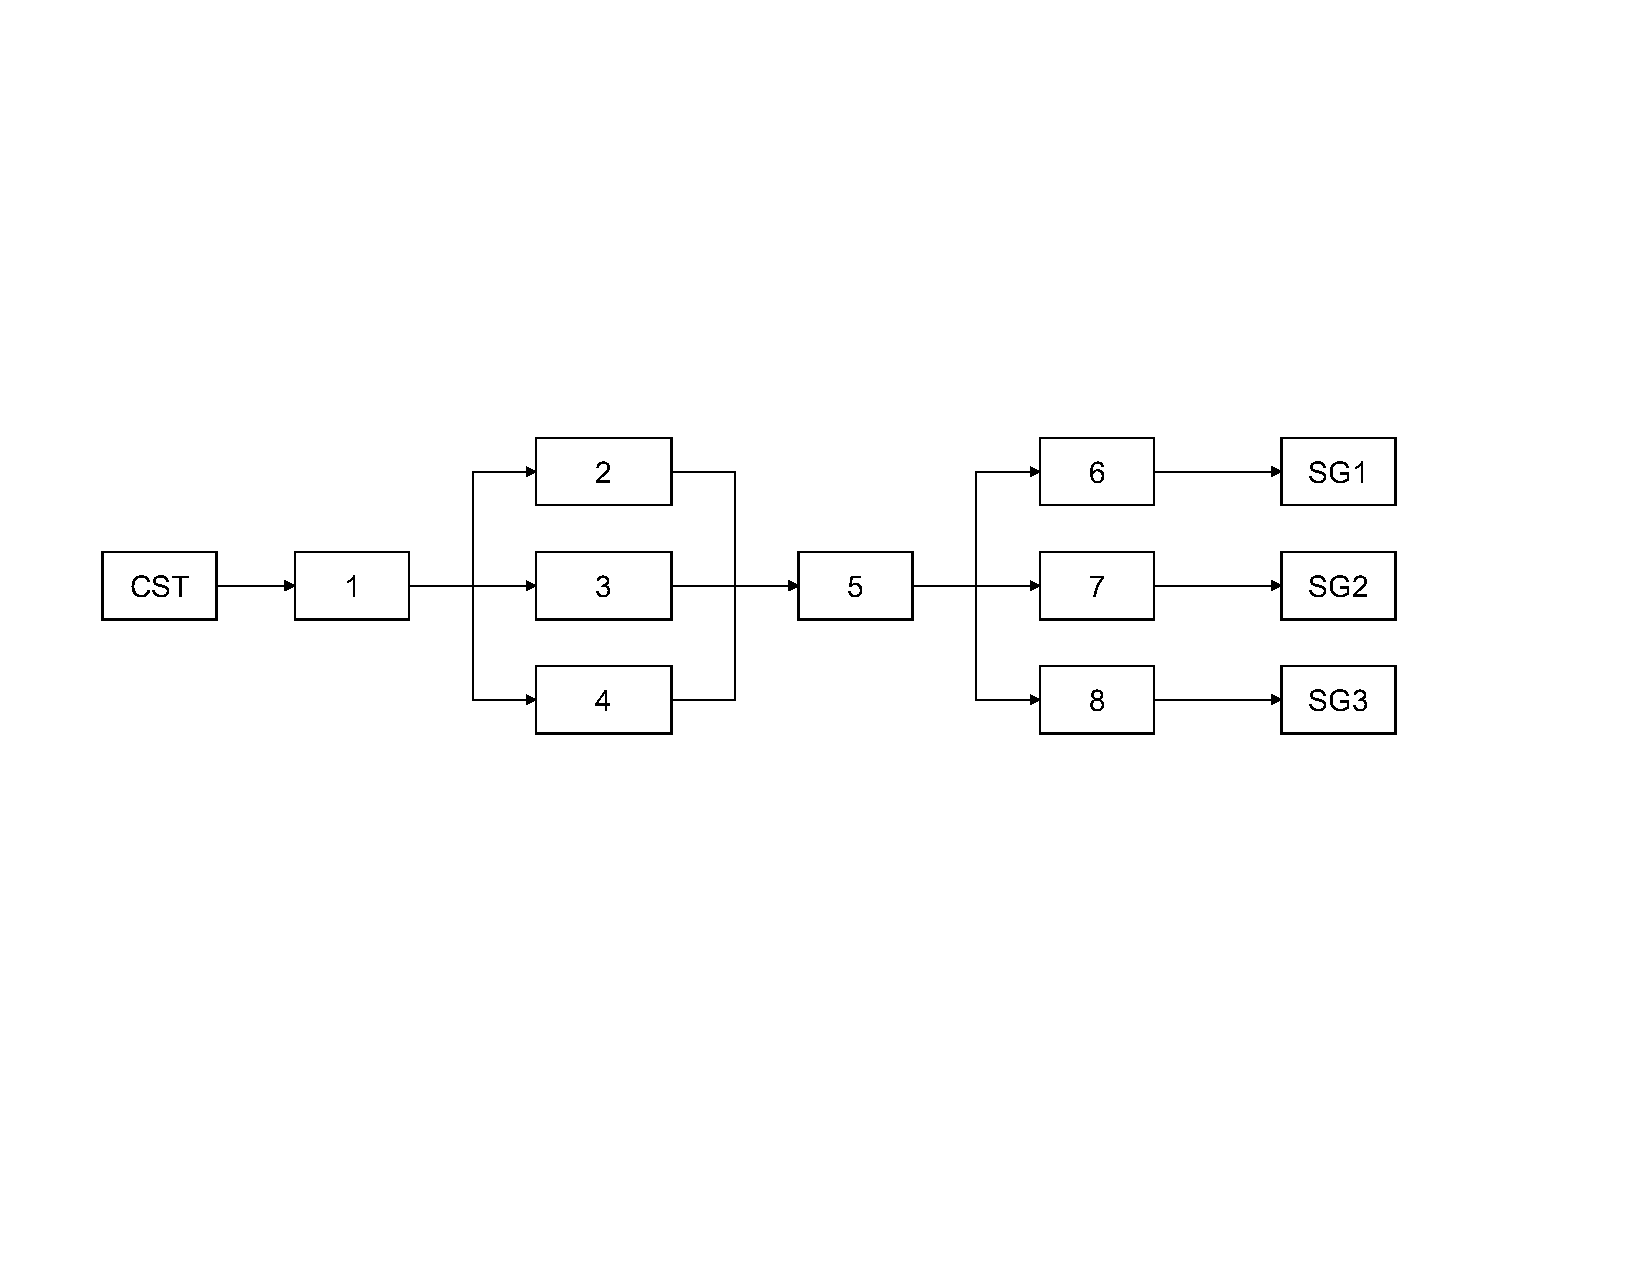
\includegraphics[scale=0.5]{RBD.pdf}}
    \caption{Example of RBD.}
    \label{fig:RBD}
\end{figure}

The FT of Fig.~\ref{fig:RBD} and defined in Listing~\ref{lst:RBDmodel} can be defined in the RAVEN input file as follows:

\begin{lstlisting}[style=XML,morekeywords={anAttribute},caption=RBD model input example., label=lst:RBD_InputExample]
  <Models>
    ...
    <ExternalModel name="graph" subType="GraphModel">
      <variables>
        status2,status3,status4,status5,
        statusSG1,statusSG2,statusSG3
      </variables>
      <modelFile>graphTest</modelFile>
      <nodesIN>CST</nodesIN>
      <nodesOUT>SG1,SG2,SG3</nodesOUT>
      <map var="status2">2</map>
      <map var="status3">3</map>
      <map var="status4">4</map>
      <map var="status5">5</map>
      <map var="statusSG1">SG1</map>
      <map var="statusSG2">SG2</map>
      <map var="statusSG3">SG3</map>
    </ExternalModel>
    ...
  </Models>
\end{lstlisting}

All the specifications of the RBD model are given in the
\xmlNode{ExternalModel} block.
Inside the \xmlNode{ExternalModel} block, the XML
nodes that belong to this models are:
\begin{itemize}
  \item  \xmlNode{variables}, \xmlDesc{string, required parameter}, a list containing the names of both the input and output variables of the model
  \item  \xmlNode{modelFile},\xmlDesc{string, required parameter}, the name of the file that provide the RBD structure
  \item  \xmlNode{nodesIN},\xmlDesc{string, required parameter}, the name of the input nodes
  \item  \xmlNode{nodesOUT},\xmlDesc{string, required parameter}, the name of the output nodes
  \item  \xmlNode{map},\xmlDesc{string, required parameter}, the name ID of the RBD node
	  \begin{itemize}
	    \item \xmlAttr{var}, \xmlDesc{required string attribute}, the ALIAS name ID of the RBD node
	  \end{itemize}
\end{itemize}

Provided this definition, the RBD model of Fig.~\ref{fig:RBD} and described in Listing~\ref{lst:RBDmodel},
the resulting model in RAVEN is characterized by these variables:
\begin{itemize}
	\item Input variables: status2, status3, status4, status5
	\item Output variable: statusSG1, statusSG2, statusSG3
\end{itemize}

\subsection{RBD model reference tests}
\begin{itemize}
	\item SR2ML/tests/test\_graphModel.xml
	\item SR2ML/tests/test\_graphModel\_TD.xml
\end{itemize}

    \section{MCSSolver}
\label{sec:MCSSolver}

This model is designed to read from file a list of Minimal Cut Sets (MCSs) and to import such Boolean logic structure as a RAVEN model.
Provided the sampled values of Basic Events (BEs) probabilities, the MCSSolver determines the probability of Top Event (TE), i.e., the union of the MCSs.
The list of MCS must be provided through a CSV file with the following format:

\begin{table}
  \begin{center}
    \caption{MCS file format.}
    \label{tab:table1}
    \begin{tabular}{c|c|c} 
      \textbf{ID} & \textbf{Prob} & \textbf{MCS}\\
      \hline
      1, & 0.01, & BE1\\
      2, & 0.02, & BE3\\
      3, & 0.03, & BE2,BE4\\
    \end{tabular}
  \end{center}
\end{table}

In this example:
\begin{itemize}
  \item three MCSs are defined: MCS1 = BE1, MCS2 = BE3 and MCS3 = BE2 and BE4 
  \item four BEs are defined: BE1, BE2, BE3 and BE4
  \item probability of TE, i.e. P(TE), is equal to: $P(TE) = P(MCS1 \cup MCS2 \cup MCS3)$
\end{itemize}

Note that the MCSSolver considers only the list of MCSs and it discards the rest of data contained in the csv file.

All the specifications of the MCSSolver model are given in the \xmlNode{ExternalModel} block. 
Inside the \xmlNode{ExternalModel} block, the XML nodes that belong to this models are:
\begin{itemize}
  \item  \xmlNode{variables}, \xmlDesc{string, required parameter}, a list containing the names of both the input and output variables of the model
  \item  \xmlNode{solverOrder},\xmlDesc{integer, required parameter}, solver order for $P(TE)$: it specifies the maximum calculation envelope 
                                                                      for $P(TE)$, i.e., the maximum number of MCSs to be considered when evaluating the 
                                                                      probability of their union
  \item  \xmlNode{topEventID},\xmlDesc{string, required parameter}, the name of the alias variable for the Top Event
  \item  \xmlNode{map},\xmlDesc{string, required parameter}, the name ID of the ET branching variable
	  \begin{itemize}
	    \item \xmlAttr{var}, \xmlDesc{required string attribute}, the ALIAS name ID of the basic event
	  \end{itemize}
\end{itemize}

An example of RAVEN input file is the following:

\begin{lstlisting}[style=XML,morekeywords={anAttribute},caption=MCSSolver model input example., label=lst:MCSSolver_InputExample]
  <Models> 
    ...
    <Models>
      <ExternalModel name="MCSmodel" subType="PRAplugin.MCSSolver">
        <variables>statusBE1,statusBE2,statusBE3,statusBE4,TOP</variables>
        <solverOrder>3</solverOrder>
        <topEventID>TOP</topEventID>>
        <map var='pBE1'>BE1</map>
        <map var='pBE2'>BE2</map>
        <map var='pBE3'>BE3</map>
        <map var='pBE4'>BE4</map>
      </ExternalModel>
    </Models>
    ...
  </Models>
\end{lstlisting}

In this case, the MCSs are written in terms of the variables BE1, BE2, BE3, and BE4.
The values of the variables pBE1, pBE2, pBE3, and pBE4 (i.e., the probability values associated to each basic event) are 
generated outside the MCSSolver model (e.g., by a sampler) and passed to the MCSSolver model in order to calculate the 
probability value of the top event (e.g., the variable TOP in the example above).
The \xmlNode{map} blocks allow the user to link the sampled probability value to the correspoding basic event.

If $solverOrder=1$ then: $P(TE) = P(MCS1)+P(MCS2)+P(MCS3)$.  
If $solverOrder=2$ then: $P(TE) = P(MCS1)+P(MCS2)+P(MCS3) - P(MCS1 MCS2) - P(MCS1 MCS3) - P(MCS2 MCS3)$.  
If $solverOrder=3$ then: $P(TE) = P(MCS1)+P(MCS2)+P(MCS3) - P(MCS1 MCS2) - P(MCS1 MCS3) - P(MCS2 MCS3) + P(MCS1 MCS2 MCS3)$

\subsection{Time dependent calculation}

The MCSSolver can also perform time dependent calculation by providing in the MultiRun step a dataObject which
contains the logic status of the Basic Events.
This dataObject contains the logical status of the the Basic Event: 0 (Basic event set to False: probability=p(BE)) 
or 1 (Basic event set to True: probability=1.0).
The format of the dataObject can be:
\begin{itemize}
  \item HistorySet: it contains the temporal profile of each basic event (e.g., BE1, BE2, BE3, and BE4) as a time 
                    series (see test\_MCSSolver_TD.xml). In this case it is needed to specify the ID of the time variable 
                    contained in the HistorySet in the \xmlNode{timeID} node.
  
   \begin{lstlisting}[style=XML,morekeywords={anAttribute},caption=Time dependent (from HistorySet) MCSSolver model input example., label=lst:MCSSolver_InputExample]
     <Models>
      <ExternalModel name="MCSmodel" subType="PRAplugin.MCSSolver">
        <variables>statusBE1,statusBE2,statusBE3,statusBE4,TOP,time</variables>
        <solverOrder>3</solverOrder>
        <topEventID>TOP</topEventID>
        <timeID>time</timeID>
        <map var='statusBE1'>BE1</map>
        <map var='statusBE2'>BE2</map>
        <map var='statusBE3'>BE3</map>
        <map var='statusBE4'>BE4</map>
      </ExternalModel>
    </Models>
  \end{lstlisting}
  
  \item PointSet: it contains the interval time (initial and final time) under which each basic event is set to 
                  True (see test\_MCSSolver_TD_fromPS.xml). As an example, the PointSet contains the IDs of the basic events
                  in the and the initial and final time as shown below:
                  
   \begin{lstlisting}[style=XML,morekeywords={anAttribute},caption= Example of PointSet for time dependent MCSSolver calculation., label=lst:MCSSolver_InputExample]
    <PointSet name="maintenanceSchedule_PointSet">
      <Input>BE</Input>
      <Output>tIn,tFin</Output>
    </PointSet>
    \end{lstlisting}
    
                  In this case, the MCSSolver requires the specification of the DataObject variables that contain the list of basic events
                  (\xmlNode{BE_ID} node) and the initial and final time values (\xmlNode{tInitial} and \xmlNode{tEnd} nodes).
                  
   \begin{lstlisting}[style=XML,morekeywords={anAttribute},caption=Time dependent (from PointSet) MCSSolver model input example., label=lst:MCSSolver_InputExample]
    <Models>
      <ExternalModel name="MCSmodel" subType="PRAplugin.MCSSolver">
        <variables>pBE1,pBE2,pBE3,pBE4,TOP,time,BE1,BE2,BE3,BE4</variables>
        <solverOrder>3</solverOrder>
        <BE_ID>BE</BE_ID>
        <tInitial>tIn</tInitial>
        <tEnd>tFin</tEnd>
        <topEventID>TOP</topEventID>
        <timeID>time</timeID>
        <map var='pBE1'>BE1</map>
        <map var='pBE2'>BE2</map>
        <map var='pBE3'>BE3</map>
        <map var='pBE4'>BE4</map>
      </ExternalModel>
    </Models>
  \end{lstlisting}
\end{itemize}

\subsection{MCSSolver model reference tests}
The following is the provided analytic test:
\begin{itemize}
  \item test\_MCSSolver.xml
  \item test\_MCSSolver_TD.xml
  \item test\_MCSSolver_TD_fromPS.xml
\end{itemize}





    \section{Reliability Models}
\label{sec:ReliabilityModels}

\textbf{Reliability Models/Functions} are the most frequently used in life data analysis
and reliability engineering. These models/functions give the probability of an component
operating for a certain amount of time without failure. As such, the reliability models
are function of time, in that every reliability value has an associated time value. In
other words, one must specify a time value with the desired reliability value. This degree
of flexibility makes the reliability model a much better reliability specification that the
MTTF (Mean Time To Failure), which represents only one point along the entire reliability
model.

\subsection{The Probability Density and Cumulative Density Functions}
From probability and statistics, given a continuous random variable $X$, we denote:
\begin{itemize}
	\item The probability density function (pdf), as $f(x)$.
	\item The cumulative density function (cdf), as $F(x)$.
\end{itemize}
If $x$ is a continuous random variable, then the probability of $x$ takes on a value in the
interval $[a,b]$ is the area under the pdf $f(x)$ from $a$ to $b$:
\begin{equation}
  P(a\leq x\leq b) = \int_{a}^{b} f(x)dx
\end{equation}
The cumulative distribution function is a function $F(x)$ of a random variable $x$, and is
defined for a number $x_0$ by:
\begin{equation}
  F(x_0) = P(x\leq x_0) = \int_{-\infty}^{x_0} f(s)ds
\end{equation}
That is, for a given value $x_0$, $F(x_0)$ is the probability that the observed value of $x$
will be at most $x_0$. The mathematical relationship between the pdf and cdf is given by:
\begin{equation}
  F(x) = \int_{-\infty}^{x} f(s)ds
\end{equation}
Conversely:
\begin{equation}
  f(x) = - \frac{dF(x)}{dx}
\end{equation}
The functions most commonly used in reliability engineering and life data analysis, namely the
reliability function and failure rate function, can be determined directly from the pdf definition,
or $f(t)$. Different distribuion exist, such as Lognormal, exponential, Weibull etc., and each of
them has a predefined $f(t)$. These distributions were formulated by statisticians, mathematicians
and engineers to mathematically model or represent certain behavior. Some distribution tend to better
represent life data and are most commonly referred to as lifetime distribution.

\subsection{The Reliability and Failure Rate Models}
Given the mathematical representation of a distribution, we can derive all of the functions that needed
for reliability analysis, i.e. reliability models/functions. This will only depend on the value of $t$
after the value of the distribution parameters are estimated from data.
Now, let $T$ be the random variable defining the lifetime of the component with cdf $F(t)$, which is the
time the component will operate before failure. The cdf $F(t)$ of the random variable $T$ is given by:
\begin{equation}
  F(t) = \int_{-\infty}^{t} f(T)dT
\end{equation}
If $F(t)$ is a differentiable function, then the pdf $f(t)$ is given by:
\begin{equation}
  f(t) = - \frac{dF(t)}{dt}
\end{equation}
The reliability function or survive function $R(t)$ of the component is given by:
\begin{equation}
  R(t) = P(T>t) = 1 - P(T\leq t) = 1-F(t)
\end{equation}
It is the probability that the component will operate after time t, sometimes called survival probability.
The failure rate of a system during the interval $[t,t+\Delta t]$ is the probability that a failure per
unit time occurs in the interval, given that a failure has not occurred prior to t, the beginning of the
interval. The failure rate function (i.e. instantaneous failure rate, conditional failure rate) of hazard
function is defined as the limit of the failure rate as the interval approaches zero. Hence
\begin{equation}
  \lambda (t)= \lim_{\Delta t\rightarrow 0} \frac{F(t+\Delta t) - F(t)}{\Delta tR(t)}
	 = \frac{1}{R(t)} \lim_{\Delta t\rightarrow 0} \frac{F(t+\Delta t) - F(t)}{\Delta t}
	 = \frac{1}{R(t)}\frac{dF(t)}{dt} = \frac{f(t)}{R(t)}
\end{equation}
The failure rate function is the rate of change of the conditional probability of failure at time $t$.
It measures the likelihood that a component that has operated up until time $t$ fails in the next
instant of time.
Generally $\lambda (t)$ is the one tabulated because it is measured experimentally and because it tends to
vary less rapidly with time than the other parameters. When $\lambda (t)$ is given, all other three
parameters $F(t)$, $f(t)$, $R(t)$ can be computed as follows:
\begin{equation}
  R(t) = \exp(-\int_{0}^{t} \lambda (s)ds)
\end{equation}
\begin{equation}
	f(t) = \lambda (t)R(t) = \lambda (t)\exp(-\int_{0}^{t} \lambda (s)ds)
\end{equation}
\begin{equation}
 	F(t) = 1 - R(t) = 1 - \exp(-\int_{0}^{t} \lambda (s)ds)
\end{equation}
The mean time between failure (MTBF) can be obtained by finding the expected value of the random variable
$T$, time to failure. Hence
\begin{equation}
  MTBF = E(T) = \int_{0}^{\infty} tf(t)dt = \int_{0}^{\infty} R(t)dt
\end{equation}

\subsection{The Lifetime Distributions or Aging Models}


\subsection{Reliability Models Reference Tests}
\begin{itemize}
	\item SR2ML/tests/reliabilityModel/test\_bathtub.xml
  \item SR2ML/tests/reliabilityModel/test\_erlangian.xml
	\item SR2ML/tests/reliabilityModel/test\_expon.xml
  \item SR2ML/tests/reliabilityModel/test\_exponweibull.xml
	\item SR2ML/tests/reliabilityModel/test\_fatiguelife.xml
  \item SR2ML/tests/reliabilityModel/test\_gamma.xml
	\item SR2ML/tests/reliabilityModel/test\_loglinear.xml
  \item SR2ML/tests/reliabilityModeltest\_lognorm.xml
	\item SR2ML/tests/reliabilityModel/test\_normal.xml
  \item SR2ML/tests/reliabilityModel/test\_powerlaw.xml
	\item SR2ML/tests/reliabilityModeltest\_weibull.xml
	\item SR2ML/tests/reliabilityModel/test\_time\_dep\_ensemble\_reliability.xml
\end{itemize}

    \section{Maintenance Models}
\label{sec:MaintenanceModels}




\textbf{Maintenance Models} are models designed to model maintenance and testing from a reliability perspective. 
These models are designed to optimize preventive maintenance at the system level. 

Two classes of models are here considered:
\begin{itemize}
	\item Operating, i.e. model \xmlAttr{type} is \xmlString{Operating}
	\item Standby, i.e. model \xmlAttr{type} is \xmlString{Standby}
\end{itemize}

The specifications of these models must be defined within a RAVEN \xmlNode{ExternalModel}. This
XML node accepts the following attributes:
\begin{itemize}
	\item \xmlAttr{name}, \xmlDesc{required string attribute}, user-defined identifier of this model.
	\nb As with other objects, this identifier can be used to reference this specific entity from other
	input blocks in the XML.
	\item \xmlAttr{subType}, \xmlDesc{required string attribute}, defines which of the sub-types should
	be used. For maintenance models, must use \xmlString{SR2ML.MaintenanceModel} as sub-type.
\end{itemize}
In the maintenance \xmlNode{ExternalModel} input block, the following XML sub-nodes are required:
\begin{itemize}
	\item \xmlNode{variable}, \xmlDesc{string, required parameter}. Comma-separated list of variable
	names. Each variable name needs to match a variable used/defined in the maintenance model or variable
	coming from other RAVEN entity (i.e. Samplers, DataObjects and Models).
	\nb For all the maintenance models, the following outputs variables would be available. If the user
	added these output variables in the node \xmlNode{variables}, these variables would be also available to
	for use anywhere in the RAVEN input to refer to the maintenance model output variables.
	\begin{itemize}
		\item \xmlString{avail}, variable that contains the calculated availability value
		\item \xmlString{unavail}, variable that contains the calculated unavailability value
	\end{itemize}
	\nb When the external model variables are defined, at run time, RAVEN initializes
	them and tracks their values during the simulation.
	\item \xmlNode{MaintenanceModel}, \xmlDesc{required parameter}. The node is used to define the maintenance
	model, and it contains the following required XML attribute:
	\begin{itemize}
		\item \xmlAttr{type}, \xmlDesc{required string attribute}, user-defined identifier of the maintenance model.
		\nb the types for different maintenance models can be found at the beginning of this section.
	\end{itemize}
\end{itemize}
In addition, if the user wants to use the \textbf{alias} system, the following XML block can be input:
\begin{itemize}
	\item \xmlNode{alias} \xmlDesc{string, optional field} specifies alias for
	any variable of interest in the input or output space for the ExternalModel.
	%
	These aliases can be used anywhere in the RAVEN input to refer to the ExternalModel
	variables.
	%
	In the body of this node the user specifies the name of the variable that the ExternalModel is
	going to use (during its execution).
	%
	The actual alias, usable throughout the RAVEN input, is instead defined in the
	\xmlAttr{variable} attribute of this tag.
	\\The user can specify aliases for both the input and the output space. As sanity check, RAVEN
	requires an additional required attribute \xmlAttr{type}. This attribute can be either ``input'' or ``output''.
	%
	\nb The user can specify as many aliases as needed.
	%
	\default{None}
\end{itemize}


\subsubsection{Operating Model}
For an operating model, the unavailability $u$ is calculated as: 
\begin{equation}
	u = lambda*Tr/(1.0+lambda*Tr) + Tpm/Tm
\end{equation}
where:
\begin{itemize}
  \item lambda: is the component failure rate
  \item Tr: mean time to repair
  \item Tpm: mean time to perform preventive maintenance
  \item Tm: preventive maintenance interval
\end{itemize}

Example XML:
\begin{lstlisting}[style=XML]
    <ExternalModel name="PMmodelOperating" subType="SR2ML.MaintenanceModel">
      <variables>lambda,Tm,avail,unavail</variables>
      <MaintenanceModel type="PMModel">
        <type>operating</type>
        <Tr>24</Tr>
        <Tpm>10</Tpm>
        <lambda>lambda</lambda>
        <Tm>Tm</Tm>
      </MaintenanceModel>
    </ExternalModel>
\end{lstlisting}

\subsubsection{Standby Model}
For an operating model, the unavailability $u$ is calculated as: 
\begin{equation}
  u = rho + 0.5*lambda*Ti + Tt/Ti + (rho+lambda*Ti)*Tr/Ti + Tpm/Tm
\end{equation}
where:
\begin{itemize}
  \item rho: failure probability per demand
  \item Ti: surveillance test interval
  \item Tr: mean time to repair
  \item Tt: test duration
  \item Tpm: mean time to perform preventive maintenance
  \item Tm: preventive maintenance interval
  \item lamb: component failure rate
\end{itemize}

Example XML:
\begin{lstlisting}[style=XML]
    <ExternalModel name="PMmodelStandby" subType="SR2ML.MaintenanceModel">
      <variables>lambda,Tm,Ti,avail,unavail</variables>
      <MaintenanceModel type="PMModel">
        <type>standby</type>
        <Tr>24</Tr>
        <Tpm>10</Tpm>
        <Tt>5</Tt>
        <rho>0.01</rho>
        <lambda>lambda</lambda>
        <Ti>Ti</Ti>
        <Tm>Tm</Tm>
      </MaintenanceModel>
    </ExternalModel>
\end{lstlisting}

    %%%%%%%%%%%%% PostProcessors %%%%%%%%%%%%%%%%
    \section{Data Classifier}
\label{sec:dataClassifier}

The \textbf{DataClassifier} post-processor is specifically used to classify the data stored in the DataObjects.
The details about this post-processor can be found in RAVEN user manual subsection \textbf{PostProcessor}
in the \textbf{Models} section.

\subsection{Data Classifier reference tests}
\begin{itemize}
	\item test\_dataClassifier\_postprocessor.xml
  \item test\_dataClassifier\_postprocessor\_HS.xml.
\end{itemize}

    \section{ET Data Importer}
\label{sec:ETdataImporter}

This post-processor is designed to import an ET as a PointSet in RAVEN.
The ET must be in: the OpenPSA format (\href{<url>}{https://github.com/open-psa}).
The details about this post-processor can be found in RAVEN user manual subsection \textbf{PostProcessor}
in the \textbf{Models} section.

\subsection{ET Importer reference tests}
\begin{itemize}
	\item test\_ETimporter.xml
	\item test\_ETimporterMultipleET.xml
	\item test\_ETimporterSymbolic.xml
	\item test\_ETimporter\_expand.xml
	\item test\_ETimporter\_DefineBranch.xml
	\item test\_ETimporter\_3branches.xml
	\item test\_ETimporter\_3branches\_NewNumbering.xml
	\item test\_ETimporter\_3branches\_NewNumbering\_expanded.xml.
\end{itemize}

    \section{FT Data Importer}
\label{sec:FTdataImporter}

This post-processor is designed to import a FT as a PointSet in RAVEN.
The FT must be in: the OpenPSA format (\href{<url>}{https://github.com/open-psa}).
The details about this post-processor can be found in RAVEN user manual subsection \textbf{PostProcessor}
in the \textbf{Models} section.

\subsection{FT Importer reference tests}
\begin{itemize}
	\item test\_FTimporter\_and\_withNOT\_embedded.xml
	\item test\_FTimporter\_and\_withNOT\_withNOT\_embedded.xml
	\item test\_FTimporter\_and\_withNOT.xml
	\item test\_FTimporter\_and.xml
	\item test\_FTimporter\_atleast.xml
	\item test\_FTimporter\_cardinality.xml
	\item test\_FTimporter\_component.xml
	\item test\_FTimporter\_doubleNot.xml
	\item test\_FTimporter\_iff.xml
	\item test\_FTimporter\_imply.xml
	\item test\_FTimporter\_multipleFTs.xml
	\item test\_FTimporter\_nand.xml
	\item test\_FTimporter\_nor.xml
	\item test\_FTimporter\_not.xml
	\item test\_FTimporter\_or\_houseEvent.xml
	\item test\_FTimporter\_or.xml
	\item test\_FTimporter\_xor.xml.
\end{itemize}

    \section{MCSImporter}
\label{MCSimporterPP}

The \textbf{MCSImporter} post-processor has been designed to import Minimal Cut Sets (MCSs) into RAVEN.
This post-processor reads a csv file which contain the list of MCSs and it save this list as a DataObject
(i.e.,  a PointSet).
The csv file is composed by three columns; the first contains the ID number of the MCS, the second one contains
the MCS probability value, the third one lists all the Basic Events contained in the MCS.
An example of csv file is shown in Table~\ref{MCScsv}.

\begin{table}[h]
    \centering
    \caption{Example of csv file which contains four MCSs.}
    \label{MCScsv}
	\begin{tabular}{c  c  c}
		\hline
		ID, & Prob, & MCS, \\
		\hline
		1.,  &  1.8E-2, &  D  \\
		2.,  &  4.0E-3, &  B \\
		3.,  &  3.0E-4, &  A,C  \\
		4.,  &  2.1E-5, &  E,C \\
		\hline
	\end{tabular}
\end{table}

The PointSet is structured to include all Basic Event, the MCS ID, the MCS probability, and the outcome of such MCS
(always set to 1).
MCS ID and MCS probability are copied directly from the csv file.
For each MCS, the Basic Events can have two possible values:
  \begin{itemize}
    \item  0: Basic Event is not included in the MCS
    \item  1: Basic Event is included in the MCS
  \end{itemize}
The PointSet generated from the csv file of Table~\ref{MCScsv} is shown in Table~\ref{PointSetMCSExpandFalse}.
\begin{table}[h]
    \centering
    \caption{PointSet generated by RAVEN for the list of MCSs shown in Table~\ref{MCScsv}.}
    \label{PointSetMCSExpandFalse}
	\begin{tabular}{c | c | c | c | c | c | c | c }
		\hline
		A & B & C & D & E & MCS\_ID & probability & out \\
		\hline
		0 & 0 & 0 & 1 & 0 & 1 & 1.8E-2 & 1 \\
		0 & 1 & 0 & 0 & 0 & 2 & 4.0E-3 & 1 \\
		1 & 0 & 1 & 0 & 0 & 3 & 3.0E-4 & 1 \\
		0 & 0 & 1 & 0 & 1 & 4 & 4.0E-3 & 1 \\
		\hline
	\end{tabular}
\end{table}

%
\ppType{MCSImporter}{MCSImporter}
%
\begin{itemize}
  \item  \xmlNode{expand},\xmlDesc{bool, required parameter}, expand the set of Basic Events by including all PRA Basic Events
  and not only the once listed in the MCSs
  \item  \xmlNode{BElistColumn},\xmlDesc{string, optional parameter}, if expand is set to True, then this node contains the
  column of the csv file which contains all the PRA Basic Events
\end{itemize}

\textbf{Example:}
\begin{lstlisting}[style=XML,morekeywords={anAttribute},caption=MCS Importer input example (no expand)., label=lst:MCS_PP_InputExample]
  <Files>
    <Input name="MCSlistFile" type="MCSlist">MCSlist.csv</Input>
  </Files>

  <Models>
    <PostProcessor name="MCSImporter" subType="SR2ML.MCSImporter">
      <expand>False</expand>
    </PostProcessor>
  </Models>

  <Steps>
    <PostProcess name="import">
      <Input   class="Files"        type="MCSlist"         >MCSlistFile</Input>
      <Model   class="Models"       type="PostProcessor"   >MCSImporter</Model>
      <Output  class="DataObjects"  type="PointSet"        >MCS_PS</Output>
    </PostProcess>
  </Steps>

  <DataObjects>
    <PointSet name="MCS_PS">
      <Input>A,B,C,D,E</Input>
      <Output>MCS_ID,probability,out</Output>
    </PointSet>
  </DataObjects>
\end{lstlisting}

\textbf{Example:}
\begin{lstlisting}[style=XML,morekeywords={anAttribute},caption=MCS Importer input example (expanded)., label=lst:MCS_PP_InputExample]
  <Files>
    <Input name="MCSlistFile" type="MCSlist">MCSlist.csv</Input>
    <Input name="BElistFile"  type="BElist" >BElist.csv</Input>
  </Files>

  <Models>
    <PostProcessor name="MCSImporter" subType="SR2ML.MCSImporter">
      <expand>False</expand>
    </PostProcessor>
  </Models>

  <Steps>
    <PostProcess name="import">
      <Input   class="Files"        type="MCSlist"         >MCSlistFile</Input>
      <Input   class="Files"        type="BElist"          >BElistFile</Input>
      <Model   class="Models"       type="PostProcessor"   >MCSimporter</Model>
      <Output  class="DataObjects"  type="PointSet"        >MCS_PS</Output>
    </PostProcess>
  </Steps>

  <DataObjects>
    <PointSet name="MCS_PS">
      <Input>A,B,C,D,E,F,G</Input>
      <Output>MCS_ID,probability,out</Output>
    </PointSet>
  </DataObjects>
\end{lstlisting}

    \section{Discrete Risk Measures}
\label{DiscreteRiskMeasures}
This Post-Processor calculates a series of risk importance measures from a PointSet.
This calculation is performed for a set of input parameters given an output target.

The user is required to provide the following information:
\begin{itemize}
   \item the set of input variables. For each variable the following need to be specified:
     \begin{itemize}
       \item the set of values that imply a reliability value equal to $1$ for the input variable
       \item the set of values that imply a reliability value equal to $0$ for the input variable
     \end{itemize}
   \item the output target variable. For this variable it is needed to specify the values of
      the output target variable that defines the desired outcome.
\end{itemize}

The following variables are first determined for each input variable $i$:
\begin{itemize}
   \item $R_0$ Probability of the outcome of the output target variable (nominal value)
   \item $R^{+}_i$ Probability of the outcome of the output target variable if reliability of the input variable is equal to $0$
   \item $R^{-}_i$ Probability of the outcome of the output target variable if reliability of the input variable is equal to $1$
\end{itemize}

Available measures are:
\begin{itemize}
   \item Risk Achievement Worth (RAW): $RAW = R^{+}_i / R_0 $
   \item Risk Achievement Worth (RRW): $RRW = R_0 / R^{-}_i$
   \item Fussell-Vesely (FV): $FV = (R_0 - R^{-}_i) / R_0$
   \item Birnbaum (B): $B = R^{+}_i - R^{-}_i$
\end{itemize}

\ppType{RiskMeasureDiscrete}{RiskMeasureDiscrete}

In the \xmlNode{PostProcessor} input block, the following XML sub-nodes are required,
independent of the \xmlAttr{subType} specified:

\begin{itemize}
   \item \xmlNode{measures}, \xmlDesc{string, required field}, desired risk importance measures
      that have to be computed (RRW, RAW, FV, B)
   \item \xmlNode{variable}, \xmlDesc{string, required field}, ID of the input variable. This
      node is provided for each input variable. This nodes needs to contain also these attributes:
     \begin{itemize}
       \item \xmlAttr{R0values}, \xmlDesc{float, required field}, interval of values (comma separated values)
          that implies a reliability value equal to $0$ for the input variable
       \item \xmlAttr{R1values}, \xmlDesc{float, required field}, interval of values (comma separated values)
          that implies a reliability value equal to $1$ for the input variable
     \end{itemize}
   \item \xmlNode{target}, \xmlDesc{string, required field}, ID of the output variable. This nodes needs to
      contain also the attribute \xmlAttr{values}, \xmlDesc{string, required field}, interval of
      values of the output target variable that defines the desired outcome
\end{itemize}

\textbf{Example:}
This example shows an example where it is desired to calculate all available risk importance
measures for two input variables (i.e., pumpTime and valveTime)
given an output target variable (i.e., Tmax).
A value of the input variable pumpTime in the interval $[0,240]$ implies a reliability
value of the input variable pumpTime equal to $0$.
A value of the input variable valveTime in the interval $[0,60]$ implies a reliability
value of the input variable valveTime equal to $0$.
A value of the input variables valveTime and pumpTime in the interval $[1441,2880]$ implies a
reliability value of the input variables equal to $1$.
The desired outcome of the output variable Tmax occurs in the interval $[2200,2500]$.
\begin{lstlisting}[style=XML,morekeywords={subType,debug,name,class,type}]
<Simulation>
  ...
  <Models>
    ...
    <PostProcessor name="riskMeasuresDiscrete" subType="RiskMeasuresDiscrete">
      <measures>B,FV,RAW,RRW</measures>
      <variable R0values='0,240' R1values='1441,2880'>pumpTime</variable>
      <variable R0values='0,60'  R1values='1441,2880'>valveTime</variable>
      <target   values='2200,2500'                  >Tmax</target>
    </PostProcessor>
    ...
  </Models>
  ...
</Simulation>
\end{lstlisting}

This Post-Processor allows the user to consider also multiple datasets (a data set for each initiating event)
and calculate the global risk importance measures.
This can be performed by:
\begin{itemize}
  \item Including all datasets in the step
\begin{lstlisting}[style=XML,morekeywords={subType,debug,name,class,type}]
<Simulation>
  ...
  </Steps>
    ...
    <PostProcess name="PP">
      <Input   class="DataObjects"  type="PointSet"        >outRun1</Input>
      <Input   class="DataObjects"  type="PointSet"        >outRun2</Input>
      <Model   class="Models"       type="PostProcessor"   >riskMeasuresDiscrete</Model>
      <Output  class="DataObjects"  type="PointSet"        >outPPS</Output>
      <Output  class="OutStreams"   type="Print"           >PrintPPS_dump</Output>
    </PostProcess>
  </Steps>
  ...
</Simulation>
\end{lstlisting}
  \item Adding in the Post-processor the frequency of the initiating event associated to each dataset
\begin{lstlisting}[style=XML,morekeywords={subType,debug,name,class,type}]
<Simulation>
  ...
  <Models>
    ...
    <PostProcessor name="riskMeasuresDiscrete" subType="SR2ML.RiskMeasuresDiscrete">
      <measures>FV,RAW</measures>
      <variable R1values='-0.1,0.1' R0values='0.9,1.1'>Astatus</variable>
      <variable R1values='-0.1,0.1' R0values='0.9,1.1'>Bstatus</variable>
      <variable R1values='-0.1,0.1' R0values='0.9,1.1'>Cstatus</variable>
      <variable R1values='-0.1,0.1' R0values='0.9,1.1'>Dstatus</variable>
      <target   values='0.9,1.1'>outcome</target>
      <data     freq='0.01'>outRun1</data>
      <data     freq='0.02'>outRun2</data>
    </PostProcessor>
    ...
  </Models>
  ...
</Simulation>
\end{lstlisting}

\end{itemize}

This post-processor can be made time dependent if a single HistorySet is provided among the other data objects.
The HistorySet contains the temporal profiles of a subset of the input variables. This temporal profile can be only
boolean, i.e., 0 (component offline) or 1 (component online).
Note that the provided history set must contains a single History; multiple Histories are not allowed.
When this post-processor is in a dynamic configuration (i.e., time-dependent), the user is required to specify an xml
node \xmlNode{temporalID} that indicates the ID of the temporal variable.
For each time instant, this post-processor determines the temporal profiles of the desired risk importance measures.
Thus, in this case, an HistorySet must be chosen as an output data object.
An example is shown below:
\begin{lstlisting}[style=XML,morekeywords={subType,debug,name,class,type}]
<Simulation>
  ...
  <Models>
    ...
    <PostProcessor name="riskMeasuresDiscrete" subType="SR2ML.RiskMeasuresDiscrete">
      <measures>B,FV,RAW,RRW,R0</measures>
      <variable R1values='-0.1,0.1' R0values='0.9,1.1'>Astatus</variable>
      <variable R1values='-0.1,0.1' R0values='0.9,1.1'>Bstatus</variable>
      <variable R1values='-0.1,0.1' R0values='0.9,1.1'>Cstatus</variable>
      <target   values='0.9,1.1'>outcome</target>
      <data     freq='1.0'>outRun1</data>
      <temporalID>time</temporalID>
    </PostProcessor>
    ...
  </Models>
  ...
  <Steps>
    ...
    <PostProcess name="PP">
      <Input     class="DataObjects"  type="PointSet"        >outRun1</Input>
      <Input     class="DataObjects"  type="HistorySet"      >timeDepProfiles</Input>
      <Model     class="Models"       type="PostProcessor"   >riskMeasuresDiscrete</Model>
      <Output    class="DataObjects"  type="HistorySet"      >outHS</Output>
      <Output    class="OutStreams"   type="Print"           >PrintHS</Output>
    </PostProcess>
    ...
  </Steps>
  ...
</Simulation>
\end{lstlisting}


    \section*{Document Version Information}
    This document has been compiled using the following version of the plug-in git repository:
    \newline
    \input{../version.tex}

    % ---------------------------------------------------------------------- %
    % References
    %
    \clearpage
    % If hyperref is included, then \phantomsection is already defined.
    % If not, we need to define it.
    \providecommand*{\phantomsection}{}
    \phantomsection
    \addcontentsline{toc}{section}{References}
    \bibliographystyle{ieeetr}
    \bibliography{user_manual}


    % ---------------------------------------------------------------------- %

\end{document}
